\documentclass{article}

\usepackage{amsmath}
\usepackage{graphicx}
\usepackage{listings}

\begin{document}

\section{Dataset Structure}
The dataset consists of 15 second recordings of pixelwise labelled RGB frames and labelled DVS events, with accompanying pose information. Data is recorded using two iniVation DAVIS 346 neuromorphic DVS cameras, which enable the simultaneous capture of binocular RGB frames and binocular pixelwise brightness changing `events'. The recordings can be categorised into various prop scenarios, in which various tool props are interacted with to varying degrees. In the first scenario, individual tool props are suspended using transparent fishing line, and perturbed in view of the cameras. In the second scenario, multiple tool props are suspended and perturbed in view of the cameras. In the third scenario, one or more tool props are held and interacted with by a human in view of the cameras. The data from each prop scenario is further categorised by the type of data contained within. Thanks to the use of iniVation DAVIS 346 cameras, our method allows the simultaneous generation of labelled RGB frame data and visual event data, so both types are included in the dataset.

Recorded data directories take the form \lstinline|./data/<category>/<sample #>|. Each directory contains three HDF5 files containing segmented RGB frames, segmented DVS events and prop pose information. For each recording, both raw and undistorted (after lens distortion correction) data is saved. RGB frame and visual event labels are integers, with $0$ meaning `background', $-1$ meaning `ambiguous' (multiple props overlap) and any $i > 0$ denoting class $i$. The fields of the RGB frame file \lstinline|frame.h5| are as follows, where $i \in \{0,...,n-1\}$ and $n = 2$ is the number of cameras:
\begin{center}
	\begin{tabular}{|c|c|}
		timestamp\_$i$           & frame timestamp (camera $i$) \\
		image\_raw\_$i$          & frame before distortion correction (camera $i$) \\
		image\_undistorted\_$i$  & frame after distortion correction (camera $i$) \\
		label\_$i$               & pixelwise frame label (camera $i$) \\
	\end{tabular}
\end{center}
The fields of the visual event file \lstinline|event.h5| are as follows:
\begin{center}
	\begin{tabular}{|c|c|}
		timestamp\_$i$        & event timestamp (camera $i$) \\
		polarity\_$i$         & event polarity (camera $i$) \\
		xy\_raw\_$i$          & event $x$ and $y$ before distortion correction (camera $i$) \\
		xy\_undistorted\_$i$  & event $x$ and $y$ after distortion correction (camera $i$) \\
		label\_$i$            & event label (camera $i$) \\
	\end{tabular}
\end{center}
Prop pose information, including translation and rotation (respectively millimetres and degrees) are stored as floating-point numbers for both global 3D tracking coordinates and camera-centric coordinates. Floating-point not-a-number indicates bad or missing data. The fields of the prop pose file \lstinline|pose.h5| are as follows:
\begin{center}
	\begin{tabular}{|c|c|}
		timestamp                           & pose timestamp \\
		extrapolated[$p$]                   & true when the pose of prop $p$ was extrapolated \\
		rotation[$p$]                       & prop $p$ rotation in global coordinates \\
		camera\_rotation\_$i$[$p$]          & prop $p$ rotation relative to camera $i$ \\
		translation[$p$][$m$]               & prop $p$ marker $m$ translation in global coordinates \\
		camera\_translation\_$i$[$p$][$m$]  & prop $p$ marker $m$ translation relative to camera $i$ \\
	\end{tabular}
\end{center}

For the sake of reproducibility, each recorded data directory also contains a JSON file linking the data to a set of OpenCV camera calibration data and calibrated Vicon to camera projection matrices which were used when collecting the data. The calibration procedure is discussed in the next section. These files are respectively held separately in directories of the form \lstinline|./camera_calibration/<date_time>| and \lstinline|./projection_calibration/<date_time>|.


\section{Calibration Procedure}
Our method uses a combination of eight Vicon Vero 2.2 tracking cameras and two iniVation DAVIS 346 DVS cameras, which are calibrated such that Vicon positions and orientations are projected accurately onto the 2D DVS image plane.To achieve this, we developed a semi-automated calibration procedure to find the translation and rotation matrices which best fit an initial trial set of synchronised Vicon and DVS data. The setup and calibration procedure of our method will be explained in this section.

We begin by discussing the issues of recording DVS event data with 3D tracking systems. A given Vicon 3D tracking system, like many other systems, works by emitting high frequency near-infrared (NIR) pulses from it's tracking cameras, and triangulating the position of returned NIR light from reflective markers. Using three or more of such markers on a single prop, the tracking system can disambiguate the orientation of the prop, providing pose information (translation and rotation). On the other hand, neuromorphic DVS cameras detect dynamic scenes by signalling changes in brightness on a per-pixel basis, enabling very low power/latency operation. Since the Vicon tracking system, by design, uses dynamic changes in NIR light to operate, it is non-trivial to use such a system in combination with DVS cameras which measure changes in brightness. To work around this issue, we manufactured a set of tracker props with built-in NIR LEDs of similar wavelength to the 780 nm light used by our Vicon tracking system. All recordings were then made with the Vicon system's NIR pulsing disabled. We eliminate the NIR light from the DVS images by attaching NIR-cut filters to the lenses.

After calibrating the DVS camera lenses (discussed later) and 3D tracking system, we begin by simultaneously collecting $100$ translation vectors from the 3D tracking system and $10000$ visual events from the DVS cameras samples of a stationary prop with 780 nm LED markers. The markers must strobe to ensure that both the tracking system and the DVS cameras can detect them (we use the Vicon Active Wand v2 NIR calibration wand set to strobe mode for this). We chose the 3D tracker marker coordinates to be the median of the Vicon translation vectors for each of the $m$ markers, and chose the 2D camera coordinates to be the centroids of a k-means clustering on the recorded DVS events with $k = m$. The DVS event k-means centroid computation was improved by filtering events through a threshold mask eroded by three pixels and dilated by ten pixels to remove noise. We then use nonlinear optimisation to compute the optimal transformation from the 3D tracking coordinates to the 2D camera plane coordinates (discussed in the next section).

Using this computed transformation, we use the numpy-stl library to project the STL mesh of the prop onto the DVS camera image plane, based on the 3D tracking system's prop translation vector, to create a segmentation mask for both RGB image and DVS event data. This approach is similar to that used by \cite{????}, however in our method we directly project the prop's STL mesh onto the camera plane, rather than the 3D prop scanned prop method used therein. While our method circumvents the need for 3D scanning hardware, some manual work is required to design and assemble accurate LED marker props with power sources. This prop label mask can be slightly dilated to fully cover the prop if rounding and calibration errors cause the mask to not fully cover the prop. During projection of the prop mesh, `bad' frames are identified on a per-prop basis by comparing the last known position and orientation to the current one, and failing if the difference is above a configurable threshold. Bad 3D tracking pose information and label masks are then linearly extrapolated, based on a configurable number of last `good' frames. While the majority of bad frames are smoothed out using this method, the prop poses and label masks are respectively set to not-a-number and all zero for the remaining larger jitters.

The tracker props we designed are available online \cite{???} in FreeCAD and STL mesh format. The code for the projection calibration procedure is available online at \cite{????}.

\section{CAD coordinate to Vicon coordinate and pose}
The entire chain of transforms from a vertex of the tool mesh in the
CAD file coordinate system to a pixel on the screens of the two DVS
cameras conceptually involves three rotation+translation transformations and a
projection+dilation+translation in the camera:
\begin{enumerate}
\item An rotation+translation transformation $\vec{y}_1 = A_1 \vec{x} +\vec{b}_1$ of the
  coordinates $\vec{x}$ in the CAD file to the coordinates $\vec{y}_1$
  of the tool if it was located at the Vicon system's origin with the
  Vicon system's $(0,0,0)$ (Tait-Bryan) angle pose. The particular Vicon origin and
  $(0,0,0)$ pose are a product of the Vicon's own calibration.
\item Another rotation+translation transformation at each time $t$ into
  $\vec{y}_2(t) = A_2(t) \vec{y}_1 + \vec{b}_2(t)$, from the vicon origin
  and $(0,0,0)$ pose to the current pose of the prop. The Tait-Bryan
  angles for the rotation matrix $A_2(t)$ and the translation $\vec{b}_2(t)$
  are provided by the vicon system as the tracked pose and position respectively.
\item A third rotation+translation transformation $\vec{z}= A_3
  \vec{y}_2 +\vec{b}_3$ into a camera-centric coordinate system with
  the origin in the (idealised) pinhole of the camera, the x and y
  axis in the orientation of the image plane and the z axis
  perpendicular to the image plane and pointing
  through the pinhole outwards.
\item the last transformation is the camera projection
  \begin{align}
    \vec{z}' = P(\vec{z}) = 
    \left(\begin{array}{c} z_1/z_3 \cdot k \\ z_2/z_3 \end{array}\right) \cdot f
    + \left(\begin{array}{c} s_x / 2 \\ s_y / 2 \end{array}\right)
  \end{align}
  where the factor $f$ involves the focal length and pixel density on
  the camera chip and $s_x$ and $s_y$ are the dimensions of the image in pixels. $k$ compensates for potential rescaling in the camera calibration method, see below.
\end{enumerate}
Additionally, we need to consider potential lens distortions of the
DVS camera lenses as we will address below.

In order to determine the first transformation, we take some
recordings of LED marker positions $\vec{y}_2(t)$ with a prop of
interest as provided by te vicon system and then
use a general optimisation technique (Nelder-Mead simplex algorithm)
to find the three Euler angles that determine $A_1$ and the three components of
$\vec{b}_1$ so that the known positions of the LED markers $\vec{x}$ in the CAD
coordinate system are mapped onto the the measured positions
$\vec{y}_2$. In order to do so we calculate
\begin{align}
  & \vec{y}_2(t) = A_2(t) \vec{y}_1 + \vec{b}_2(t) \\
  \Leftrightarrow \quad & A_2^T(t) (\vec{y}_2 - \vec{b}_2(t)) = \vec{y}_1 =
  A_1 \vec{x} +\vec{b}
\end{align}
and hence minimise the cost function
\begin{align}
  C= \sum_{i,t} \left(A_2^T(t) (\vec{y}_2^{(i)}(t) - \vec{b}_2(t)) -
  \vec{x}^{(i)}\right)^2
\end{align}
where $i$ enumerates the different LED markers of the prop and $t$ the
time frames taken for this calibration step. $A_2(t)$ is obtained as
the rotation matrix determined by the Vicon provided ``Tait-Bryan''
pose and $\vec{b}_2$ as the Vicon provided prop location.

\section{Vicon coordinate to DVS camera transform}
Our approach for this step has been to do two calibrations:
\begin{enumerate}
\item Camera calibration: This is done with OpenCV and takes care of the lens distortions so that the corrected camera frames are according to a ``normal'' or rectilinear camera projection. The hope was that this would essentially be the equivalent of the the pinhole camera projection. Note that this transformation does involve slightly non-uniform rescaling of images, where the x-direction is slightly stretched compared to y (this will be an important detail below)
\item Based on the assumption of a pinhole camera, the transformation from an arbitrary coordinate system in 3D (e.g. the reference frame of the global positioning system, hereafter referred to as the ``vicon system''). We will discuss below how these assumptions worked out.
\end{enumerate}

The camera calibration is described elsewhere (ref).
For the camera projection, we started with the knowledge that the
transformation is composed of a rotation+translation transformation and a simple pinhole projection, followed by transformation from mm to pixels and a move of the origin from the centre of teh image to the upper left corner. To make things interpretable, we explicitly use the focal length in the projection, transform mm to pixels and translate the image frame origin from the centre of the picture to the upper left corner. From these transformations, the mm to pixel and move of the origin are based on camera data and not fitted. The rotation, translation, focal length and potential relative scaling of x versus y due to the camera calibration procedure (8 parameters) are determined through the fitting procedure.
The general form of the transformation is
\begin{align}
  \vec{z} &= \frac{1}{a} \left(\begin{array}{cc} k & 0 \\ 0 & 1 \end{array}\right) P(A_3\cdot \vec{y}_2 + \vec{b}_3) + \frac{d}{2} \\
  P(\vec{y}) &= \frac{1}{y_3}f \vec{y}  
\end{align}
where $a= 18 \mu m/\text{pixel}$ is the spacing of pixels on the image chip, $P$ is the Projection with focal length $f$, $\vec{d}= (346, 260)$ is the image dimension in pixels, and $A_3$ and $\vec{b}_3$ denote the (unknown) rotation+translation transformation from the vicon refrence frame into the camera reference frame. The latter has axes x to the right of the image, y downwards and z from the image plane through the pinhole outwards. $k$ is the rescaling of the x direction to counteract potential distortions from the amera calibration procedure.

In order to determine the unknown parameters of $A_3$, $\vec{b}_3$, $f$ and $k$, we have taken a simple calibration approach: We place the vicon calibration wand that has 5 LEDs in different positions and orientations in the camera view area and acquire vicon coordinates of the LEDs and simultaneously detect the LEDs from the DVS events. There is a processing step where multiple DVS events are clustered with k-means clustering into 5 clusters to find the best estimate for the position $\vec{z}$ of the LEDs in the DVS image. Then, the main calibration step is to use a general optimization method to minimise the mean squared distance of $\vec{z}$ and the positions obtained by using equations (\ref{eqn1},\ref{eqn2}) on the simultaneaously acquired vicon coordinates $\vec{y}_2$. In practice we use the Nelder-Mead simplex algorithm as implemented in the scipy.optimize.minimize function.

\begin{figure}
  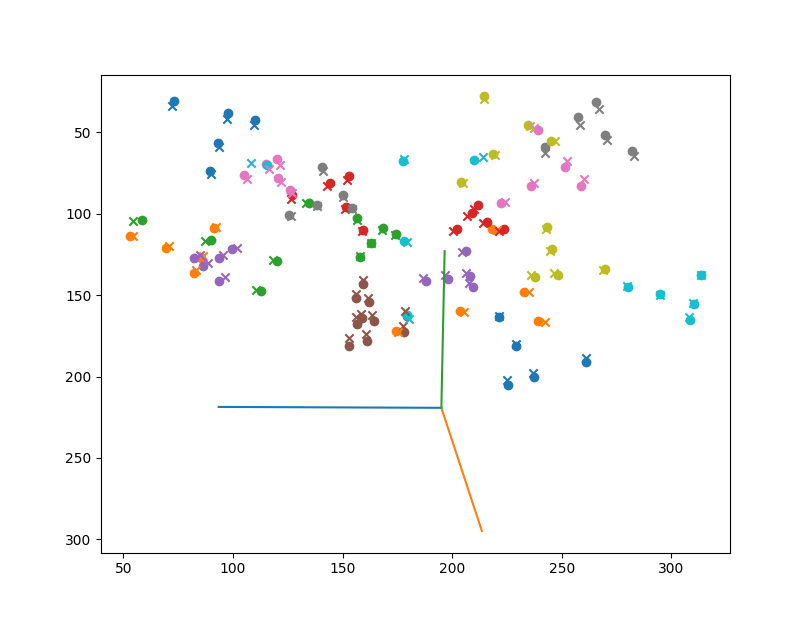
\includegraphics[width=\textwidth]{figure_match_euler.png}
  \caption{\label{figure3} Fitting results after the correction factor fo the focal length was introduced.}
\end{figure}

Subsequently, we have used the transformation to project the 3D meshes of tools from the positions and poses detected by the vicon sytem onto the DVS frames with good success. Figure \ref{figure3} illustrates the quality of this calibration procedure for an example calibration data set. The residual error was RMS$= 13.56$.
 As the Nelder-Mead algorithm is a simple hill-climbing algorithm, the quality of fits could be affected by being stuck in a local minimum. We therefore tried several runs with different parameter combinations using the ``basinhopping'' algorithm. We typically observed no further improvements.

\subsection{Camera-centric position and pose}
In order to create training data for regressors that predict position and pose of a tool based on DVS data, we need to record position and pose relative to the DVS camera reference frame. Otherwise, the training data, and hence the models, would depend on the (quite likely changing) camera position and orientation, as well as the Vicon calibration data at any particular time.

In order to obtain the camera-centric data, we can get the position information simply by translating the CAD file origin using our full chain of transformations $\vec{z_0}= A_3(A_2(A_1 \vec{0}+ \vec{b}_1)+\vec{b}_2)+\vec{b}_3)= A_3(A_2(\vec{b}_1)+\vec{b}_2)+\vec{b}_3$. For the pose, we don't need to consider the translations and hence just determine the Euler angles of the combined rotation $A_3 \cdot A_2(t) \cdot A_1$.

\section{Conventions}
We are using proper Euler angles in the $z_\alpha \rightarrow x'_\beta \rightarrow z''_\gamma$ convention of rotating first around the $z$ axis by $\alpha$ (counter-clockwise is $\alpha > 0$ when looking towards the origin), then around the new $x'$ axis by $\beta$ and then around the new $z''$ axis by $\gamma$. The angles are constrained to $\alpha, \gamma \in [-\pi, \pi]$ and $\beta \in [0, \pi]$.

The Vicon positioning software uses Tait-Bryan angles with convention $x_\alpha \rightarrow y'_\beta \rightarrow z''_\gamma$ and, like for us, counter-clockwise corresponds to angle $ > 0$ when looking towards the origin. The angles are contained as $\alpha, \gamma \in [-\pi, \pi]$ and $\beta \in [-\frac{\pi}{2}, \frac{\pi}{2}]$.
\end{document}
